\section{Numerical}

\subsection{Cable nets}
For the first experiment we will consider $4$ free nodes and the following parameters:

$4$ fixed nodes $p^{(1)} = (5,5,0),\; p^{(2)} = (-5,5,0),\; p^{(3)} = (-5,-5,0),\; p^{(4)} = (5,-5,0)$

$k=3,\quad \el = 3 \quad \forall \quad (i,j) \in \mathcal{E}, \quad m_i g = \frac{1}{6}, \quad i= 5,6,7,8$

$\mathcal{E} = \{(1,5),\;(2,6),\;(3,7),\;(4,8),\; (5,6),\; (6,7),\; (7,8),\; (8,5) \}$

This problem has a analytical solution for the free nodes:

$ x^{(5)} = (2,2,-\frac{3}{2}),\;x^{(6)} = (-2,2,-\frac{3}{2}),\;x^{(5)} = (-2,-2,-\frac{3}{2}),\;x^{(5)} = (2,-2,-\frac{3}{2})$

\begin{figure}
    \centering
    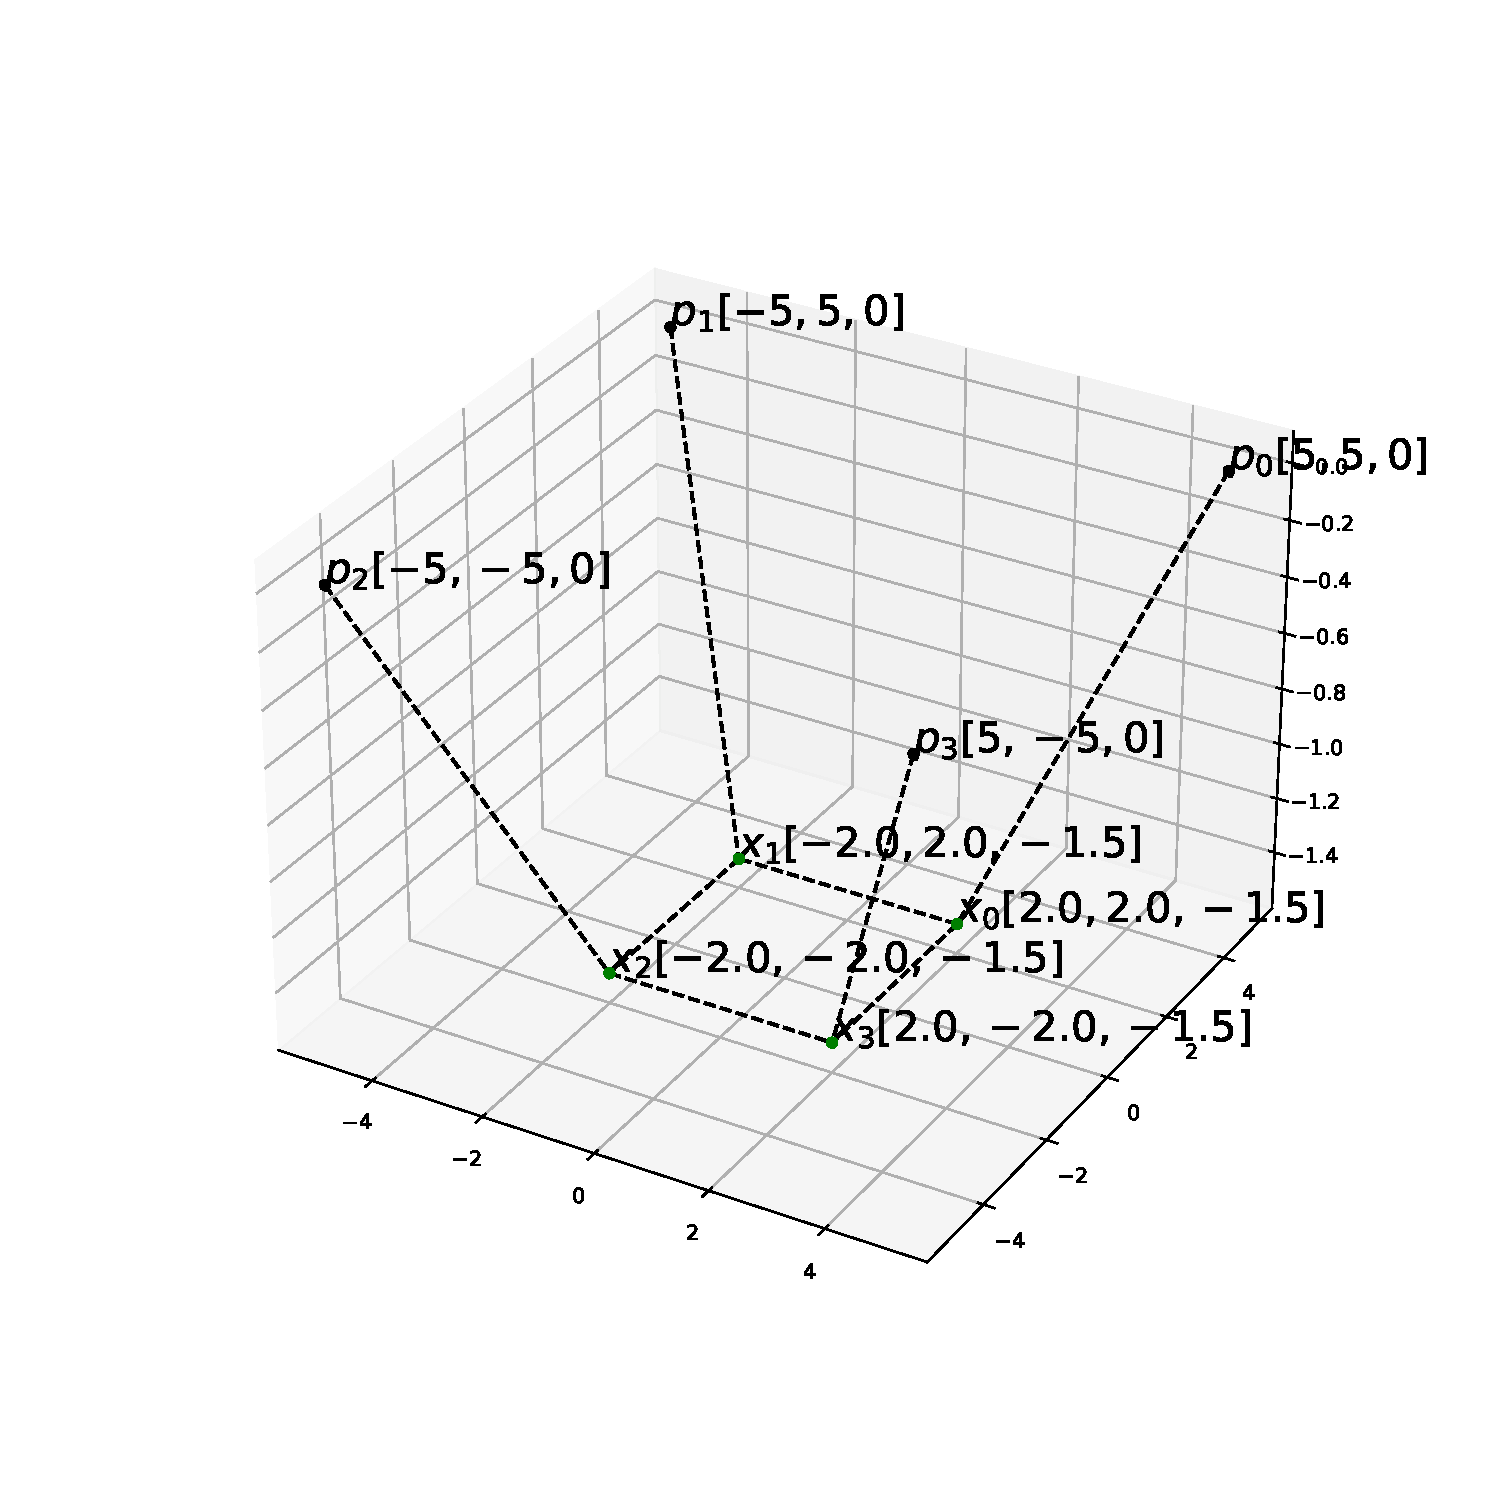
\includegraphics[width=0.6\columnwidth]{Bilder/P25.pdf}
    \caption{Cable net structure}
    \label{P25}
\end{figure}
We see from \eqref{P25} that we indeed reach this configuration of nodes. 

\textbf{Noe om at den ender opp i samme løsning uansett startkonfigurasjon?}

\subsection{Tensegrity domes}
We now consider bars as well, and will use the $4$ fixed nodes $p^{(1)} = (1,1,0),\; p^{(2)} = (-1,1,0),\; p^{(3)} = (-1,-1,0),\; p^{(4)} = (1,-1,0), $ and the following parameters:

\begin{equation}
    \begin{gathered}
    \ell_{15} = \ell_{26} = \ell_{37} = \ell_{48} = 10 \qquad \ell_{18} = \ell_{25} = \ell_{36} = \ell_{47} = 8 \qquad \ell_{56} = \ell_{67} = \ell_{78} = \ell_{58} = 1\\
    c=1, \quad k= 0.1, \quad g \rho = 0,\quad m_i g = 0, \quad i = 5,6,7,8
    \end{gathered}
\end{equation}


\begin{figure}
    \centering
    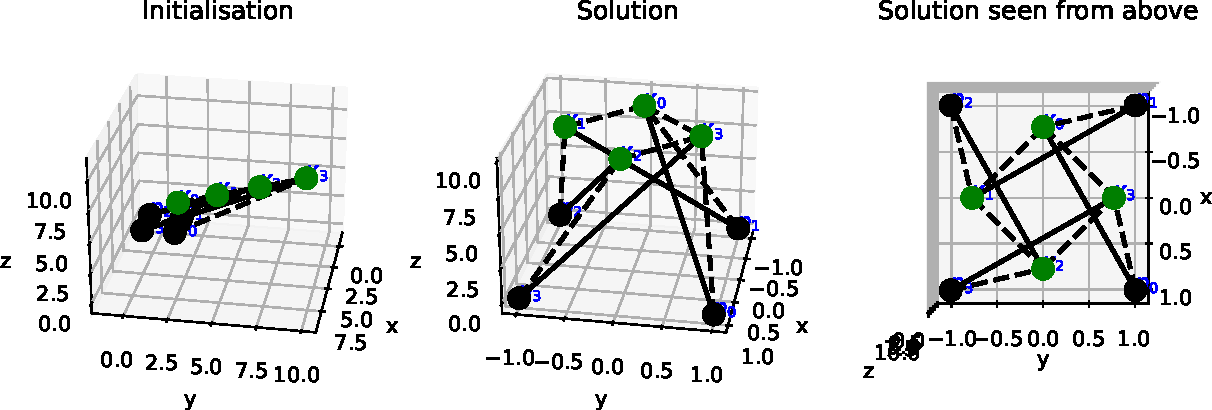
\includegraphics[width=0.6\columnwidth]{Bilder/P69.pdf}
    \caption{Caption}
    \label{P69}
\end{figure}

Again, we have an analytical solution to this problem, namely \\$x^{(5)} = (-s,0,t),x^{(6)} = (0,-s,t),x^{(7)} = (s,0,t),x^{(8)} = (0,s,t), $ with $s \approx 0.70970 \quad \text{and} \quad t \approx 9.54287$